\documentclass{iiufrgs}
\usepackage[utf8]{inputenc}   % pacote para acentuação
\usepackage{graphicx}           % pacote para importar figuras
\usepackage{times}              % pacote para usar fonte Adobe Times
\usepackage{framed}             % para exemplos e TODOs
\usepackage{biblatex}           % para referências bibliográficas
\usepackage{xcolor}             % cores
\usepackage{hyperref}           % referências
\usepackage{amsmath}
\usepackage{float}

\colorlet{shadecolor}{orange!15}

\title{Laboratório 1}
\author{}{Thiago Bell}

\addbibresource{report.bib}

\begin{document}
\maketitle

\setcounter{chapter}{1}

\section{Tarefa}
Implementar uma heap n-ária e usá-la ao implementar o algoritmo de Dijkstra. Verificar desempenho da heap e do algoritmo de Dijsktra e compará-los com as previs\~oes teóricas.
Os testes presentes no plano de teste sugerido foram utilizados neste trabalho.

\section{Implementaç\~ao}
Os algoritmos foram implementados em C++. A heap utiliza um vetor da standard library da linguagem para o armazenamento da árvore de forma eficiente. Os grafos s\~ao representados por lista de adjacências.
\section{Ambiente de Teste}
Os experimentos foram realizados usando um processador Intel i7 2600k acompanhado de 8 GiB de RAM. O sistema operacional utilizado foi Ubuntu Linux 16.04.
\section{Análise de Complexidade da Heap}
A complexidade teórica das operaç\~oes da heap foram comparadas com os resultados de experimentos. Os quais respeitam a expectativa teórica. 
\subsection{Avaliaç\~ao das Operaç\~oes de Inserç\~ao}
Fixando-se o valor $n = 2^{27}-1$, adicionou-se $n$ elementos na heap com chaves no intervalo de $[n,1]$.  Como se usou uma heap de grau 2, isso corresponde a 27 níveis completos na árvore. Ao adicionar os elementos, após inserir $2^{i}-1$ chaves, mede o tempo $T_i$ e o número de swaps $I_i$ onde $0<=i<=27$. A complexidade dessa operaçao é de $O(2^i ~ \dot i)$. Com isso pode-se estimar o custo $E = 2^i ~ \dot i$ para cada $i$. Na figura \ref{fig:insert1} pode-se ver o número de swaps e E em funç\~ao de $2^i$. Para ficar claro que a complexidade é respeitada, a curva E*15 mostra os valores de $E$ multiplicados por uma constante. Na figura \ref{fig:insert2}, mostra-se a raz\~ao entre o tempo obtido experimentalmente e o custo teórico. Nota-se que a curva para valores maiores de $2^i$ tende a um valor constante o que indicaria que o tempo e o custo est\~ao crescendo na mesma taxa.

Considerando as duas comparaç\~oes, conclui-se que a implementaç\~ao da inserç\~ao na heap respeita a complexidade do algoritmo.


\begin{figure}[H]
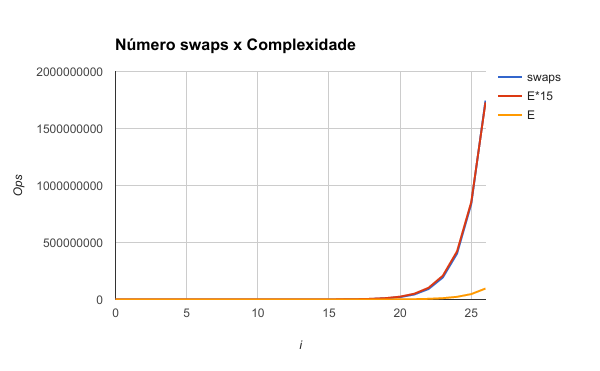
\includegraphics[width=0.75\linewidth]{insert1}
\centering
\caption{}{}
\label{fig:insert1}
\end{figure}
\begin{figure}[H]
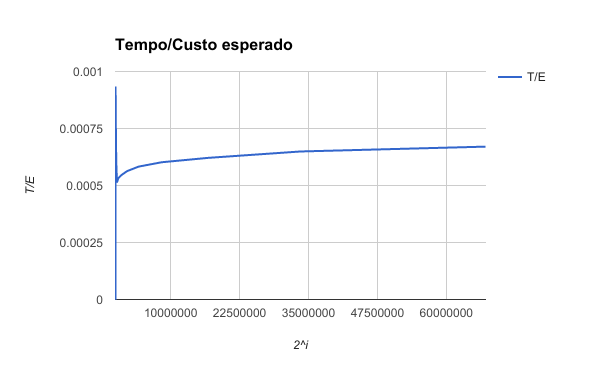
\includegraphics[width=0.75\linewidth]{insert2}
\centering
\caption{}{}
\label{fig:insert2}
\end{figure}
\subsection{Avaliaç\~ao das Operaç\~oes de Atualizaç\~ao}
Considerando-se uma variável $i$, $2^i -1$ chaves s\~ao inseridas com valor de $2^i +1$. Em seguida, $2^i$ chaves com valor $2^i +2$ s\~ao adicionadas. Medindo-se o tempo e o número de swaps, as chaves com valor, $2^i +2$ s\~ao atualizadas para valores decrescentes no intervalo $[2^i, 1]$. As operaç\~oes de atualizaç\~ao começam por $2^i$ e a cada operaç\~ao seguinte esse valor é decrescido por 1. 

O custo teórico esperado também é de $E = 2^i \dot i$. Ao comparar com o número de swaps obtido para cada iteraç\~ao, percebeu-se que estes valores s\~ao iguais. Logo, pelo menos em número de swaps, a complexidade é obedecida. No entanto, ao comparar o tempo de execuç\~ao, o resultado obtido foi uma reta inclinada o que indicaria que o tempo de execuç\~ao cresce mais que o esperado.

\begin{figure}[H]
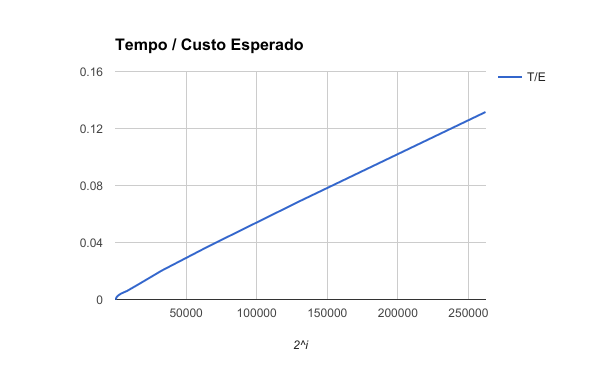
\includegraphics[width=0.75\linewidth]{update}
\centering
\caption{}{}
\label{fig:update1}
\end{figure}

\subsection{Avaliaç\~ao das Operaç\~oes de Remoç\~ao}
Para um valor $i$, $2^{i} - 1$ chaves com valor aleatórios s\~ao adicionados. Depois, $2^{i - 1}$ chaves s\~ao removidas. O tempo de execuç\~ao e o número de swaps foram medidos para cada i. O custo teórico dessas operaç\~oes é de $E = 2^i \dot i$. Na figura \ref{fig:delete1} é comparado esse custo com o número de swaps. De forma análoga a feita anteriormente, também se multiplicou o valor de E por uma constante. A comparaç\~ao do tempo de execuç\~ao com E pode ser vista na figura \ref{fig:delete2}. A convergência a um valor indica que o tempo de execuç\~ao cresce conforme a complexidade do algoritmo.

\begin{figure}[H]
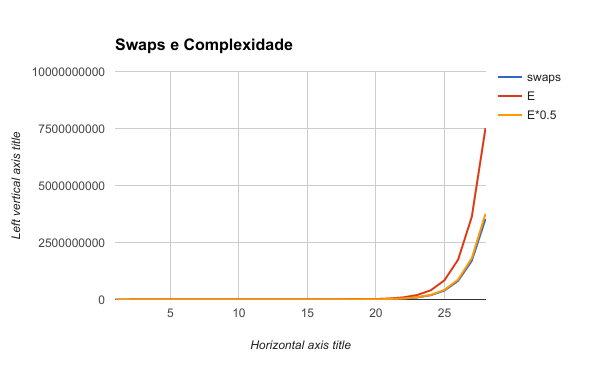
\includegraphics[width=0.75\linewidth]{delete1}
\centering
\caption{}{}
\label{fig:delete1}
\end{figure}

\begin{figure}[H]
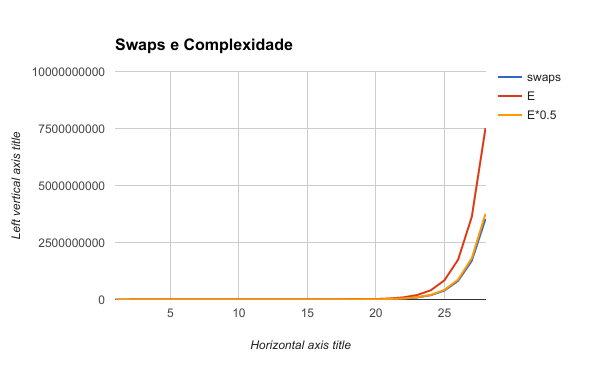
\includegraphics[width=0.75\linewidth]{delete1}
\centering
\caption{}{}
\label{fig:delete2}
\end{figure}

\section{Análise de Complexidade do Algoritmo de Dijkstra}
\subsection{Variando o número de Arestas}
Fixou-se o número de vértices em $2^{15}$ e variou-se o número de arestas entre $2^{18}$ e $2^{24}$. Ao comparar o tempo de execuç\~ao com o custo teórico de $E = (n+m)*log(n)$, obteve-se uma convergência a um valor constante como pode ser visto na figura \ref{fig:dij_vertex}. Os números de inserts e deletes foram menores ou iguais ao de vértices e o de update menores ou iguais ao de arestas.
\begin{figure}[h!]
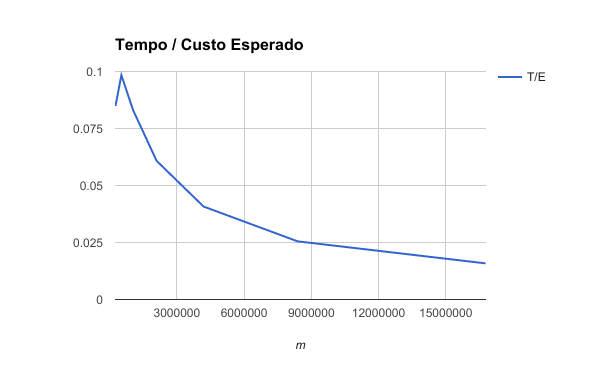
\includegraphics[width=0.75\linewidth]{dijkstra_fixedvertex}
\centering
\caption{}{}
\label{fig:dij_vertex}
\end{figure}

\subsection{Variando o número de Vértices}
Fixou-se o número de arestas em $2^{20}$ e variou-se o número de vértices entre $2^{11}$ e $2^{18}$. O custo teórico é o mesmo do caso anterior, $E = (n+m)*log(n)$. Encontrou-se um problema onde o grafo se tornavo excessivamente esparso e o algoritmo de dijkstra encerrava sem percorrer parte significante do grafo. Poucas amostras foram obtidas como fica evidente na figura \ref{fig:dij_edge}.
\begin{figure}[h!]
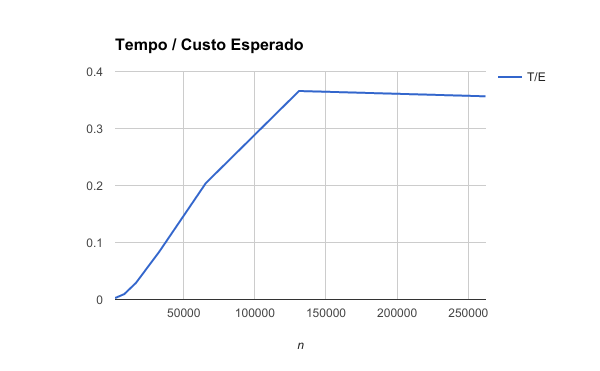
\includegraphics[width=0.75\linewidth]{dij_fixed_edge}
\centering
\caption{}{}
\label{fig:dij_edge}
\end{figure}


\section{Verificando a implementaç\~ao de Dijkstra com grandes instâncias}
Testou-se a implementaç\~ao do algoritmo com duas instâncias conforme recomendado no plano de teste. Para o caso de teste consistindo da rede completa dos Estados Unidos provida na definiç\~ao do trabalho, obteve-se um tempo médio de execuç\~ao de 169 segundos e consumo de memómia máximo de 3.64 GB. Para a rede de Nova York, foram 1.83 segundos e 43.7 MB de memória.


\section{Testando Grau Ótimo da Heap}
Testou-se a implementaç\~ao da heap variando-se o grau da mesma e usando as redes de Nova York e dos Estados Unidos assim como outras geradas aleatóriamente geradas com uma vers\~ao modificada do algoritmo gerador oferecido. Um comportamento interessante foi obtido. Para as redes reais, os resultados foram melhores para graus 4 e 8. Entretando, para as artificiais a tendência foi de quanto maior o grau da heap, melhor o desempenho ao executar o algoritmo de Dijkstra. A figura \ref{fig:narity} mostra os resultados. Os tempos de execuç\~ao de cada grafo foram normalizados em relaç\~ao ao tempo médio obtido para aquela rede. Acredita-se que esse comportamento, possa ser explicado pela aleatoriedade na atribuiç\~ao de grafos o que resulta numa topologia diferente.
\begin{figure}[h!]
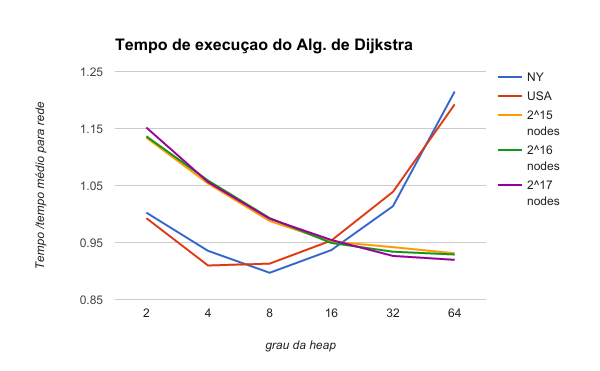
\includegraphics[width=0.75\linewidth]{narity}
\centering
\caption{}{}
\label{fig:narity}
\end{figure}

\section{Conclus\~ao}
Excluindo-se o caso onde n\~ao se obteve resultados experimentais satisfatórios e o onde a medida de tempo divergiu da de swaps, as implementaç\~oes dos algoritmos respeitaram a complexidade teórica dos mesmos.
\end{document}